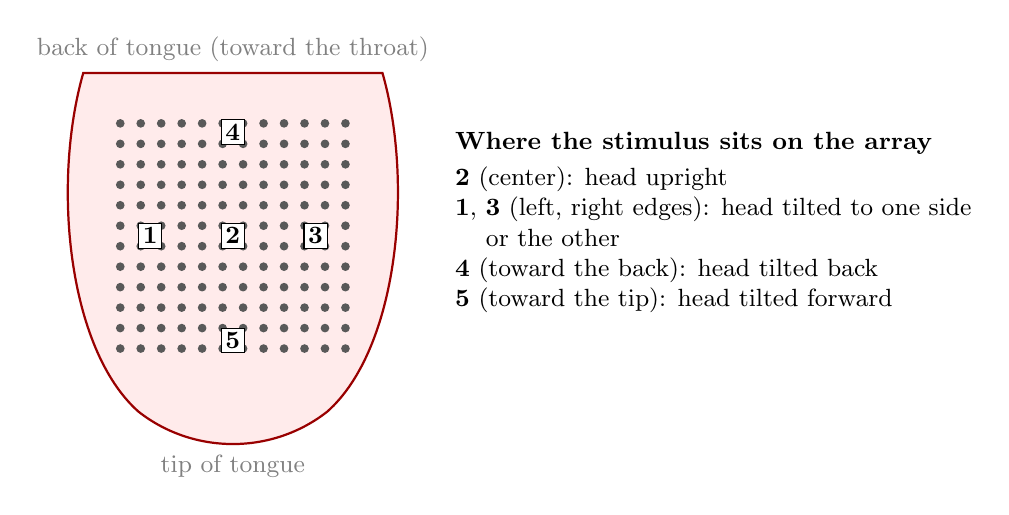
\begin{tikzpicture}[font=\small]
  % tongue outline (back of the tongue at the top, tip at the bottom)
  \filldraw[fill=red!8, draw=red!60!black, thick]
    (-1.9,1.9) .. controls (-2.3,0.5) and (-2.1,-1.6) .. (-1.2,-2.4)
    .. controls (-0.5,-2.95) and (0.5,-2.95) .. (1.2,-2.4)
    .. controls (2.1,-1.6) and (2.3,0.5) .. (1.9,1.9) -- cycle;
  \node[gray] at (0,2.2) {back of tongue (toward the throat)};
  \node[gray] at (0,-3.1) {tip of tongue};
  % electrode grid
  \foreach \i in {0,...,11} {
    \foreach \j in {0,...,11} {
      \fill[gray!70!black] (-1.43+0.26*\i, -1.6+0.26*\j) circle (0.055);
    }
  }
  % numbered stimulus positions
  \foreach \n/\x/\y in {4/0/1.15, 1/-1.05/-0.17, 2/0/-0.17, 3/1.05/-0.17, 5/0/-1.5} {
    \node[draw, fill=white, inner sep=1.5pt, font=\small\bfseries] at (\x,\y) {\n};
  }
  % key
  \node[anchor=west, align=left] at (2.7,0) {%
    \textbf{Where the stimulus sits on the array}\\[2pt]
    \textbf{2} (center): head upright\\
    \textbf{1}, \textbf{3} (left, right edges): head tilted to one side\\
    \hspace{1.2em}or the other\\
    \textbf{4} (toward the back): head tilted back\\
    \textbf{5} (toward the tip): head tilted forward};
\end{tikzpicture}
